\documentclass{standalone}
\usepackage{tikz}
\begin{document}
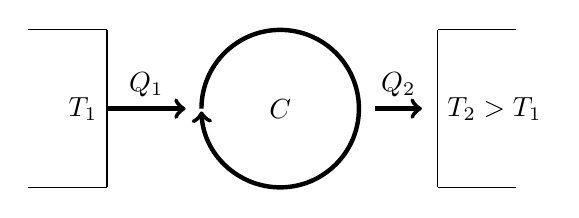
\begin{tikzpicture}[scale=2]
    \draw[-](-0.5,0.5)--(0,0.5);
    \draw[-](-0.5,-0.5)--(0,-0.5);
    \draw[-](0,0.5)--(0,-0.5);
    \node[left]at(0,0){$T_1$};
    \draw[->,ultra thick](0,0)--(0.5,0)node[midway, above]{$Q_1$};
    \node[]at(1.1,0){$C$};    
    \draw[->,ultra thick](0.6,0)arc(180:-178:0.5);
    \draw[->,ultra thick](1.7,0)--(2,0)node[midway, above]{$Q_2$};
    \draw[-](2.1,-0.5)--(2.1,0.5);
    \node[right]at(2.1,0){$T_2>T_1$};
    \draw[-](2.1,0.5)--(2.6,0.5);
    \draw[-](2.1,-0.5)--(2.6,-0.5);
\end{tikzpicture}
\end{document}